\documentclass[11pt,a4paper]{article}
\usepackage[utf8]{inputenc}
\usepackage[french]{babel}
\usepackage[T1]{fontenc}
\usepackage{amsmath}
\usepackage{amsfonts}
\usepackage{amssymb}
\usepackage{fourier}
\usepackage{graphicx}
\usepackage{framed}
\usepackage[left=2cm,right=2cm,top=2cm,bottom=2cm]{geometry}
\usepackage{listings}
\usepackage{xcolor}

\definecolor{pgreen}{rgb}{0,0.5,0}
\definecolor{Zgris}{rgb}{0.87,0.85,0.85}

%%configuration de listings
\lstset{
language=c++,
basicstyle=\ttfamily\small, %
identifierstyle=\color{pgreen}, %
keywordstyle=\color{blue}, %
stringstyle=\color{black!60}, %
commentstyle=\it\color{green!95!yellow!1}, %
columns=flexible, %
tabsize=2, %
extendedchars=true, %
showspaces=false, %
showstringspaces=false, %
numbers=left, %
numberstyle=\tiny, %
breaklines=true, %
breakautoindent=true, %
captionpos=b
}

\lstset{backgroundcolor=\color{Zgris}}





\newsavebox{\BBbox}
\newenvironment{DDbox}[1]{
\begin{lrbox}{\BBbox}\begin{minipage}{\linewidth}}
{\end{minipage}\end{lrbox}\noindent\colorbox{Zgris}{\usebox{\BBbox}} \\
[.5cm]}

%Document Information
\title{Rapport de Laboratoire d'électronique digitale de 3BE : Programmation d'un PIC18 en Langage C}
\date{\today}
\author{Selleslagh Tom, Wéry Benoît}

\begin{document}
	\maketitle
	\textbf{Thème} : La notion de convertisseur analogique-numérique
	\section{Introduction}
\paragraph{}
Le but de ce laboratoire est de comprendre le concept de conversion analogique/numérique, au moyen d'une carte de développement dont le microprocesseur est de la famille des PIC18F.
\paragraph{}
Dans la quasi-totalité des cas, le monde physique est perçu par des signaux analogiques (le son, la lumière, ...). Le traitement de ces signaux peut se faire de manière analogique ou numérique. Cependant, le recours au traitement numérique offre plusieurs avantages :
\begin{itemize}
\item facilité de stockage de l'information
\item reproductibilité des traitements du signal d'entrée
\item réalisation plus aisée des fonctionnalités de traitements complexes
\item ...
\end{itemize}
\paragraph{}
L'interface couramment utilisée pour faire le lien entre ces deux mondes est le Convertisseur Analogique Numérique (CAN) ou Analogic Digital Converter (ADC) en anglais.
%http://www.mines-stetienne.fr/~dutertre/documents/cours_convertisseurs.pdf
	\section{Principe général}
L'objectif de ce laboratoire est d'utiliser l'ADC que contient le PIC18F et de convertir la tension d'entrée en une valeur numérique codée sur 10 bits et stockée dans une variable de 16 bits. Il sera donc important de spécifier si l'on désire aligner nos bits à gauche ou à droite.(cf FIG \ref{align})

\begin{figure}
\begin{center}
\begin{framed}
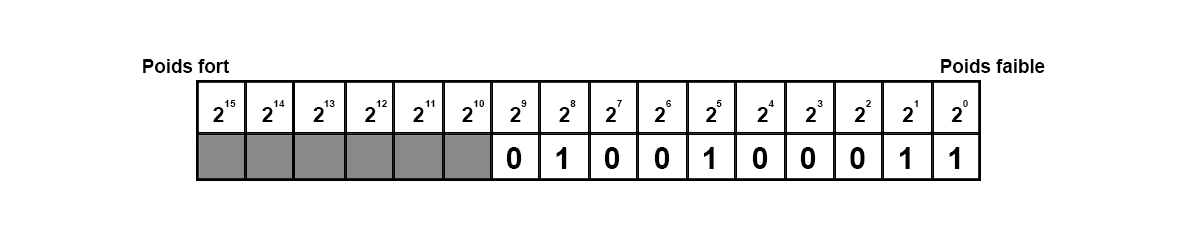
\includegraphics[scale=0.8]{images/aligndroite.png}
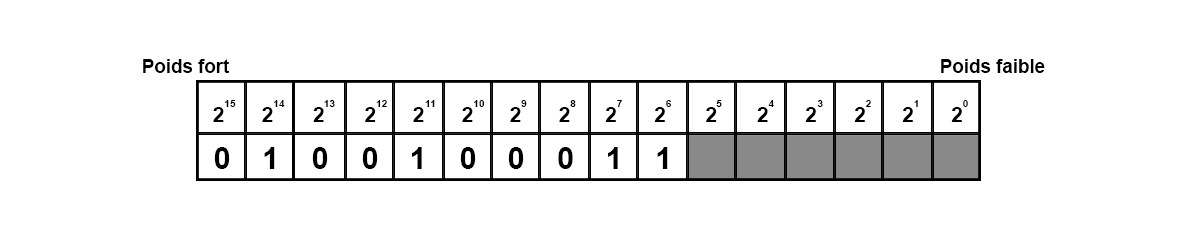
\includegraphics[scale=0.8]{images/aligngauche.png}
\caption{Alignement des 10 bits encodés dans la variable sur 16 bits}
\label{align}
\end{framed}
\end{center}
\end{figure}

\subsection{Paramètres de l'ADC}

\subsubsection*{Tensions de références}
Bornes de tension entre lesquelles le PIC18F convertira le signal d'entrée. Si la tension mesurée se situe entre les deux bornes, alors la valeur digitale retournée sera calculée proportionnellement aux valeurs binaires extrêmes.(Dans ce laboratoire nous choisirons $V_{SS}$ et $V_{DD}$ comme tensions de références basse et haute)
\subsubsection*{Temps de conversion Analogique $\rightarrow$ Digital  ($T_{AD}$)}
Le $T_{AD}$  est le temps minimum nécessaire à l'ADC pour mesurer un bit. Le $T_{AD}$ se configure comme un multiple en puissance de 2 de la période d'oscillation de la clock du PIC18F ($T_{osc} = 25ns$).
\subsubsection*{Temps d'acquisition ($T_{ACQ}$)}
Le $T_{ACQ}$ est le temps minimum nécessaire pour que le condensateur CHOLD se charge. Le $T_{ACQ}$  se configure comme un multiple de 2 du $T_{AD}$. 
 
	\section{Programmation}
\label{programmation}
Nous ne présenterons ici que le \textbf{paramétrage} de l'ADC, le codage de son utilisation sera explicité au moyen d'un exemple dans la section \ref{notion}
\paragraph{}
Il existe deux méthodes pour configurer les registres de l'ADC :

\subsection{Sans libraire}
Il s'agit de modifier directement les bits de configuration dans les registres adéquats. Le paramétrage de l'ADC se fera sur les registres ADCON0, ADCON1 et ADCON2.

\paragraph{Tensions de références :} on configure pour que les tensions de références soient  $V_{SS}$ et $V_{DD}$


\begin{lstlisting}
ADCON1bits.VCFG0 = 0;
ADCON1bits.VCFG1 = 0;
\end{lstlisting}

\paragraph{Alignement des bits encodés:} alignement à droite.
\begin{lstlisting}
ADCON2bits.ADFM = 1;
\end{lstlisting}


\paragraph{\textbf{$T_{AD}$}:} paramétrage pour un $T_{AD}$ = $\frac{F_{OSC}}{16}$
\begin{lstlisting}
ADCON2bits.ADCS2 = 1;
ADCON2bits.ADCS1 = 0;
ADCON2bits.ADCS0 = 1;
\end{lstlisting}

\paragraph{\textbf{$T_{ACQ}$}:} paramétrage pour un $T_{ACQ}$ = 6 $T_{AD}$
\begin{lstlisting}
ADCON2bits.ACQT2 = 0;
ADCON2bits.ACQT1 = 1;
ADCON2bits.ACQT0 = 1;
\end{lstlisting}


\paragraph{Choix de l'entrée analogique :} dans cette configuration on choisi l'entrée AN0 que l'on place en "mode" analogique. 
 
\begin{lstlisting}
ADCON0bits.CHS0 = 0;
ADCON0bits.CHS1 = 0;
ADCON0bits.CHS2 = 0;
ADCON0bits.CHS3 = 0;
ADCON1bits.PCFG0 = 0;
\end{lstlisting}

\subsection{Avec la libraire}
En utilisant la libraire XC8 nous pouvons utiliser les fonctions \textbf{OpenADC()} et \textbf{ SetChanADC()} pour réaliser ces mêmes opérations.

\paragraph{}
\begin{lstlisting}
OpenADC(ADC_FOSC_16 & ADC_RIGHT_JUST & ADC_6_TAD,
            ADC_REF_VDD_VSS,
            0);

SetChanADC(ADC_CH0);
ADCON1bits.PCFG0 = 0;
\end{lstlisting}



	\section{Notions avancées}
\label{notion}
Un exemple d'utilisation de l' ADC est la gestion des signaux PWM (Pulse Width Modulation) ou  MLI (Modulation de Largeur d'Impulsions) en français. 
\paragraph{}
Le principe général de la modulation PWM est qu'en appliquant une succession d'états discrets pendant des durées bien définies, on peut générer des signaux continus. La valeur moyenne du signal obtenu est alors égale au rapport cyclique du module PWM:   $\text {rapport cyclique} =  \frac{\text{Temps haut}}{\text{Période}}$ . Un exemple pour une tension d'entrée de 3V vous est présenté à la FIGURE \ref{pwm}.



\begin{figure}[h]
\begin{center}
\begin{framed}
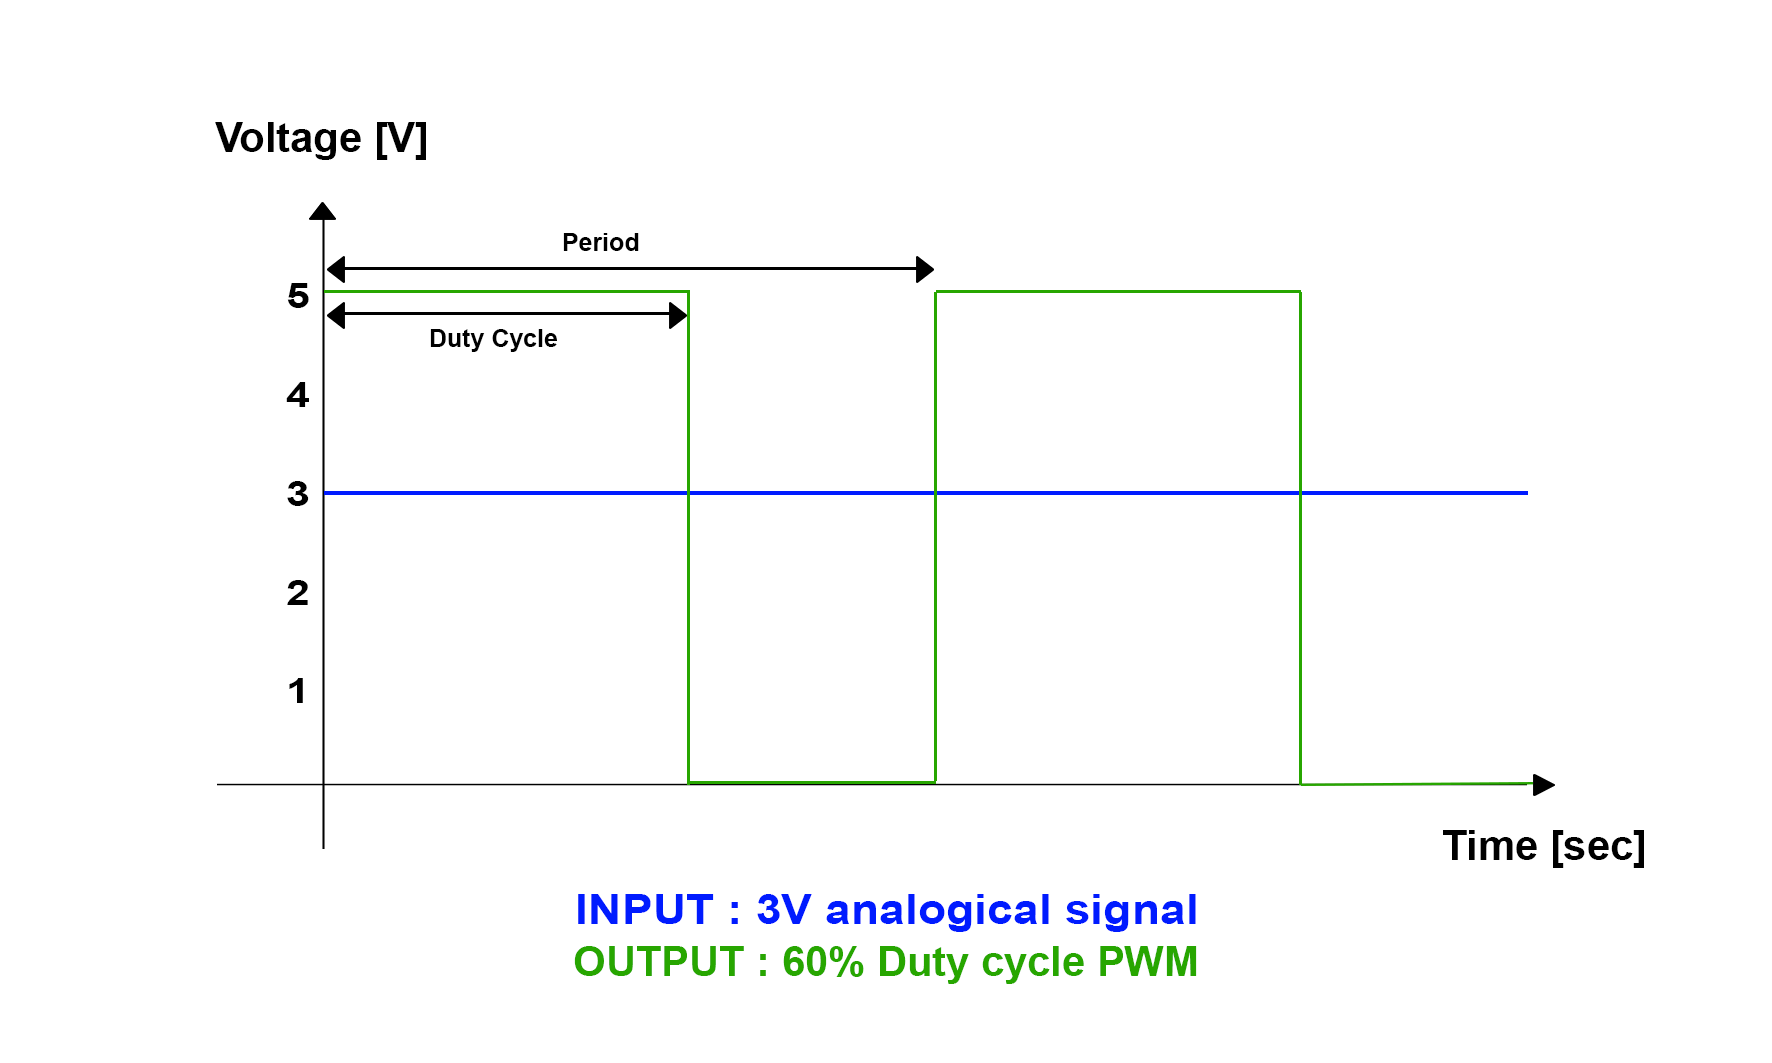
\includegraphics[scale=0.8]{images/pwm.png}
\caption{Transformation d'un signal analogique en signal PWM de tension équivalente}
\label{pwm}
\end{framed}
\end{center}
\end{figure}

\paragraph{}
Une application concrète de ces notions est le contrôle d'un moteur DC au moyen d'un signal PWM. Le moteur est placé dans un montage en pont H dont l'ouverture et la fermeture des interrupeurs est commandée par le signal PWM (voir FIGURE \ref{pontH}). Afin de gérer le sens de rotation du moteur ainsi que sa vitesse, on utilise un potentiomètre et un convertisseur Analogique-Numérique. Celui-ci aura alors pour fonction de traduire la valeur analogique de la tension lue sur le potentiomètre en un rapport cyclique pour le module PWM. Ainsi, par exemple,  si le potentiomètre est mis sur la résistance minimale, l'ADC convertira cette valeur en un rapport cyclique minimum et le moteur sera à basse vitesse\footnote{Nb: nous ne développeront cependant pas le code pour ce genre d'application, car il s'agit d'une utilisation directe d'une PWM, mais indirecte d'un ADC.}.

\begin{figure}[h]
\begin{center}
\begin{framed}
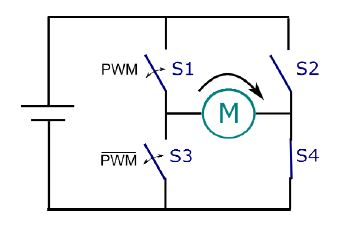
\includegraphics[scale=0.8]{images/pontH.jpg}
\caption{Contrôle d'un moteur DC via un montage en pont H}
\label{pontH}
\end{framed}
\end{center}
\end{figure}

\paragraph{}
Utilisation du signal numérique de sortie de l'ADC pour créer une PWM, via les librairies du compilateur XC8:

\paragraph{Création de la PWM} paramétrage de la période\footnote{
le calcul de la durée de la période de la PWM se fait grâce à la formule $period =[(period ) + 1] x 4 x TOSC x TMR2 prescaler$. Cette valeur sera renseignée comme paramètre de la fonction OpenPMMx() et du mode.}
\begin{lstlisting}
OpenPWM1(0xFF);
SetOutputPWM1(SINGLE_OUT, PWM_MODE_1);
\end{lstlisting}

\paragraph{Conversion} On suppose l'ADC correctement paramétré pour lire la tension sur le potentiomètre (voir Section \ref{programmation}).
Les fonctions \textbf{ConvertADC()}, \textbf{BusyADC()} et \textbf{ReadADC()} permettent respectivement : 
\begin{itemize}
\item de demander à l'ADC de lancer une mesure
\item de vérifier si il a fini de convertir la tension analogique
\item de lire le résultat de la conversion
\end{itemize}

\begin{lstlisting}
ConvertADC();
while(BusyADC());
value = ReadADC();
\end{lstlisting}

\paragraph{Redirection de la sortie numérique de l'ADC vers la PWM}.
\begin{lstlisting}
SetDCPWM1(value);
\end{lstlisting}

\paragraph{Fermeture de l'ADC à la fin du programme}.
\begin{lstlisting}
CloseADC();
\end{lstlisting}


	\section{Conclusion}
	\section*{Annexes}
\textbf{Sources:}
\begin{itemize}
\item \url{https://fr.wikipedia.org/wiki/Convertisseur_analogique-num.}
\item Note de laboratoires 2 et 3 d'électroniques Numériques, ECAM , 2016.
\end{itemize}
\end{document}
